\section{问题四：实时波动电价下的购电与储能调控}
\label{sec:q4}

\subsection{问题分析}

问题四将固定分时电价改为实时波动电价，并要求分别重新计算问题二和问题三。此时购电量与购电时刻共同决定实际费用，储能既用于缓冲负载和光伏预测误差，也用于降低高价时段的紧急购电费用。

本文以决策时可获得的历史电价预测当日价格，按预测电价制定购电计划和储能动作，交付时按附件4中的实际电价结算。问题四-2保留问题二的零点全天计划和边际价值DP；问题四-3保留问题三的融合预报、双向策略调整、六小时分段更新和递减价值DP。

图\ref{fig:q4-workflow}概括两类任务从电价预测、购电规划和储能控制到费用核验的流程。

\begin{figure}[H]
    \centering
    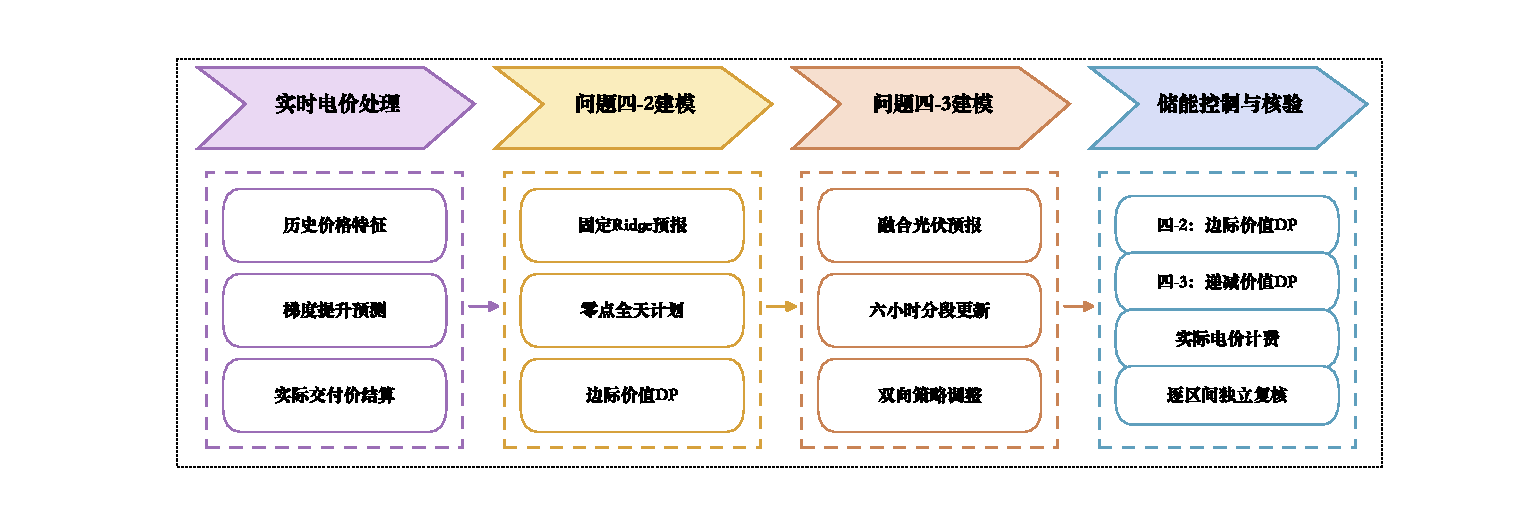
\includegraphics[width=\textwidth,trim=28mm 8mm 24mm 8mm,clip]{figures/q4/flowchart4.pdf}
    \caption{问题四流程图}
    \label{fig:q4-workflow}
\end{figure}

\subsection{实时电价预测}

\subsubsection{预测变量与信息范围}

记$p_{kt}$为第$k$日第$t$个区间的实际电价，$\widehat p_{kt}$为当日0:00可获得的预测电价。预测模型仅使用第$k$日以前的电价记录，包括昨日同刻、近三次同星期同刻、近期均值以及时刻、星期和年内周期特征。采用直方图梯度提升回归，每7日利用最近最多60日的历史样本重新拟合，模型参数在2月至12月的计算过程中保持预先设定。

设决策日以前的信息集合为$\mathcal F_{k,0}$，则
\begin{equation}
    \widehat p_{kt}=f_{\theta_k}(\mathcal F_{k,0},t),
    \qquad
    \theta_k\ \text{仅由第$k$日以前的数据估计}.
    \label{eq:q4-price-forecast}
\end{equation}
当日规划使用预测电价，交付时按实际电价$p_{kt}$结算。采用相同的历史信息范围，昨日同刻、同星期同刻和近期均值三种基准方法的MAE分别为0.0843、0.0466和0.0534元/kWh，RMSE分别为0.1238、0.0663和0.0710元/kWh。直方图梯度提升模型在2025年2月至12月48,096个区间上的MAE为0.0399元/kWh，RMSE为0.0545元/kWh，两项误差均为四种方法中的最小值，因此用于问题四的电价预测。

\subsubsection{预测价决策与实际价结算}

问题四-2在0:00形成全天普通购电量$q_{kt}^{0}$，剩余缺口由紧急购电$u_{kt}$补足，实际费用为
\begin{equation}
    C_{4-2}=\sum_k\sum_{t=0}^{T-1}
    \left(p_{kt}q_{kt}^{0}+5p_{kt}u_{kt}\right).
    \label{eq:q4-2-cost}
\end{equation}

问题四-3沿用式\eqref{eq:q3-windows}的发布时刻。令$a_{k,t}$、$b_{k,t}$分别为最终策略相对零点计划的增购量和减购量。0:00基础购电费只支付一次，减购时退回原购电费并支付50\%违约费，实际费用为
\begin{equation}
 C_{4-3}=\sum_k\sum_{t=0}^{T-1}
 \left(p_{kt}q_{kt}^{0}+1.5p_{kt}a_{kt}-0.5p_{kt}b_{kt}+5p_{kt}u_{kt}\right).
 \label{eq:q4-3-cost}
\end{equation}

\subsection{购电与储能模型}

\subsubsection{问题四-2的全天计划}

问题四-2保持问题二的固定Ridge负载、光伏预测和0.8分位数安全余量。将问题二目标函数中的固定电价替换为$\widehat p_{kt}$，在电池功率、容量、效率和供需平衡约束下求解全天计划。全天采用零点确定的普通购电计划，实际运行阶段使用边际价值DP决定是否放电；紧急购电全部用于补足当前负载缺口。

\subsubsection{问题四-3的分段更新}

问题四-3沿用问题三的预测与控制参数。0:00将附件3预报与历史预测按0.56和0.44融合，形成全天基础购电计划；6:00、12:00和18:00利用最新预报重新规划至当天24:00。第$r$次重规划只确认$\mathcal I_r$内的购电量，$\mathcal H_r\setminus\mathcal I_r$内的结果用于估计储能对后续时段的作用。

零点计划日末储电量设为2400\,kWh。日内规划以6000\,kWh为软参考量，允许相对零点策略增购或减购，并按预测电价计算规划目标。储能控制采用问题三的50\,kWh网格递减价值DP，后续价值权重为0.95；在四个发布时间分别重建价值函数，每次执行随后36个区间。实际日末储电量直接作为次日初值。

\subsection{模型求解}

\textbf{Step 1：电价预测。} 每日0:00由此前已完成日期的数据生成144个区间的预测电价，作为当日规划的价格输入。

\textbf{Step 2：购电规划。} 问题四-2仅在0:00求解全天计划；问题四-3在四个发布时间重新求解剩余时段，并只确认到下一发布时间的购电调整。

\textbf{Step 3：储能控制。} 问题四-2使用边际价值DP；问题四-3在每个发布时间依据最新光伏预报重建递减价值DP。所有动作均使用连续储电量，电池状态跨日传递。

\textbf{Step 4：费用复算。} 采用实际交付电价逐区间计算普通购电费、策略调整费用净额和紧急购电费，并独立复核供需平衡、储电量递推、容量、功率及充放电互斥约束。

\subsection{求解结果}

\subsubsection{两类任务的年度结果}

评估期为2025年2月1日至12月31日，共334天。表\ref{tab:q4-main}给出两类任务在实际年末储电量条件下的结果。

\begin{table}[H]
\centering\small
\caption{实时波动电价下的年度费用与运行结果}
\label{tab:q4-main}
\renewcommand{\arraystretch}{1.18}
\begin{tabularx}{\textwidth}{@{}>{\columncolor{white}[0pt][\tabcolsep]}lRRRRR>{\columncolor{white}[\tabcolsep][0pt]}R@{}}
\toprule
\rowcolor{paperpale}
任务与控制方法 & 基础购电费/万元 & 策略调整费用净额/万元 & 紧急购电费/万元 & 总费用/万元 & 紧急电量/kWh & 年末储电量/kWh\\
\midrule
问题四-2，边际价值DP & 1421.2538 & 0 & 36.3918 & 1457.6456 & 60,665.46 & 6,018.42\\
\rowcolor{paperstripe}
问题四-3，递减价值DP & 1345.1474 & 24.1991 & 25.3294 & 1394.6759 & 44,687.76 & 2,448.95\\
\bottomrule
\end{tabularx}
\end{table}

问题四-2的总费用为1457.6456万元，其中紧急购电费36.3918万元。紧急购电发生在119天的708个十分钟区间，将同日连续区间合并后得到253次事件。

问题四-3的总费用为1394.6759万元，其中基础购电费1345.1474万元、策略调整费用净额24.1991万元、紧急购电费25.3294万元。紧急购电发生在164天的759个十分钟区间，合并后得到298次事件。

图\ref{fig:q4-annual-comparison}汇总问题二至问题四的年度费用分解和紧急购电量。

\begin{figure}[H]
\centering
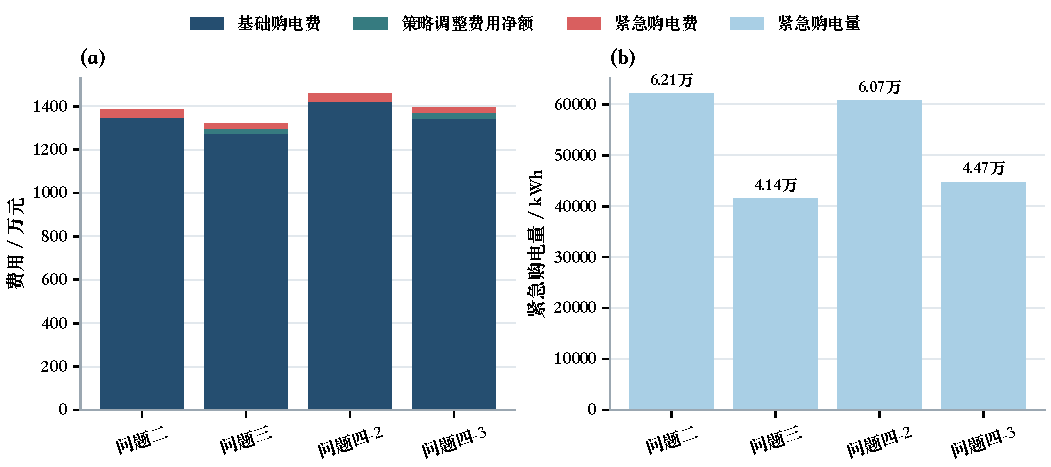
\includegraphics[width=\textwidth]{figures/q4/q4_annual_comparison.pdf}
\caption{问题二至问题四主方案的年度费用构成与紧急购电量}
\label{fig:q4-annual-comparison}
\end{figure}

图\ref{fig:q4-annual-comparison}表明，问题三和问题四-3通过日内预报调整降低紧急购电量。波动电价增大了补购时点的费用差异，问题四-2使用边际价值DP保留储能至较高预测电价时段；问题四-3进一步利用融合预报和双向策略调整降低基础购电费用。

\subsubsection{储能控制与网格精度对照}

问题四-2在统一6000\,kWh年末储电量下比较贪心控制与边际价值DP。问题四-3保持模型不变，将储电量网格由50\,kWh细化为25\,kWh，结果见表\ref{tab:q4-controller}。

\begin{table}[H]
\centering\small
\caption{储能控制方法与网格精度对照}
\label{tab:q4-controller}
\renewcommand{\arraystretch}{1.18}
\begin{tabularx}{\PaperTableCompactWidth}{@{}>{\columncolor{white}[0pt][\tabcolsep]}lRR>{\columncolor{white}[\tabcolsep][0pt]}R@{}}
\toprule
\rowcolor{paperpale}
对照项目 & 对照费用/万元 & 采用方案费用/万元 & 费用差/万元\\
\midrule
问题四-2：贪心/边际价值DP & 1460.3750 & 1458.0700 & 2.3049\\
\rowcolor{paperstripe}
问题四-3：25/50\,kWh网格 & 1394.6809 & 1394.6759 & 0.0050\\
\bottomrule
\end{tabularx}
\end{table}

问题四-2中，边际价值DP较贪心控制节省2.3049万元。以配对逐日费用差为样本，采用7日连续块重采样10000次，随机种子取2026，所得95\%区间为$[0.7065,4.5125]$万元。问题四-3细化网格后费用仅变化49.50元，年末储电量和紧急购电量保持不变，50\,kWh网格能够满足本题精度要求。

\subsubsection{两类任务的费用比较}

问题四-3比问题四-2少支出62.9697万元，紧急购电量减少15,977.70\,kWh。两类任务同时改变光伏预报来源、购电调整方式和储能控制参数，该差额反映题目要求的两套完整策略的综合变化。

\subsection{模型检验}

对两类主结果的48,096个区间进行独立复算。供需平衡残差上界为$2.3\times10^{-12}$\,kWh，累计储电量递推误差低于$4.8\times10^{-11}$\,kWh，跨日连续残差为0。所有区间均满足1200--10800\,kWh容量边界和833.33\,kWh单区间充放电上限，充电与放电互斥，紧急购电全部用于补足负载缺口。逐项费用复算误差低于$1.5\times10^{-11}$元。

\subsection{结论}

实时波动电价下，问题四-2采用零点全天计划和边际价值DP，总费用为1457.6456万元；问题四-3采用融合光伏预报、六小时分段更新、双向策略调整和递减价值DP，总费用为1394.6759万元。两类策略均按预测电价决策，并按实际交付电价结算。
